\chapter{This is the Chapter Title}\label{ch:chapter}
\pagenumbering{arabic}\setcounter{page}{1}

This is how a chapter looks like. Note that in the first \textit{numbered} chapter you write (the introduction, for instance), you have to include the command:
\begin{verbatim}
	\pagenumbering{arabic}\setcounter{page}{1}
\end{verbatim}
otherwise, the page numbering will be shown in Roman numerals and the page counter won't be reset.

\section{This is the Section Title}\label{sec:section}

This is how a section looks like. 

\subsection{This is the Subsection Title}\label{subsec:subsection}

This is how a subsection looks like. 

\subsubsection{This is the Subsubsection Title}

This is how a subsubsection looks like. 

\paragraph{This is the Paragrah Title} And finally, this is how a paragraph looks like. Notice how both subsubsections and paragraphs are not numbered, but can be used to give more structure to your document. \\
\\
Now, we can explore some of the features mentioned in the \texttt{README.md} file. \\
\indent First, let's talk math. You can use the \verb|\v{}| command, to show a vector $\v{x}$, or with a greek symbol $\v{\Gamma}$. When compared to the scalar versions of the same letters (i.e., $x$ and $\Gamma$), the vectors will appear as bold and not italic. For the three-dimensional column vector, you can use the \verb|\vthree{}{}{}| command, and \verb|\quaternion| to show the quaternion vector:
\[ \vthree{x}{y}{z} = \quaternion \]
Since quaternions have 4 elements, the above expression makes no sense, but gladly this is not my thesis. There are also commands for derivatives, such as:
\[ \dif{x} \qquad \d{x}{t} \qquad \dd{x}{t} \qquad \pd{x}{t} \qquad \pdd{x}{t} \qquad \dpar{g}{x}{2} \]
You can also use the \verb|f{}| command to print a function. For instance, you can have $\f{f}{x}$ or $\f{\v{X}}{y}$. Finally, you can use the \verb|\chem{}| command to show chemical formulas, such as \chem{H_2O} or \chem{C_6H_{12}O_6}. \\
\\
Then, we can talk about the mouse-hover tags. Make sure to be using Adobe Reader to see these effects. The first command is the \verb|\abbr{}| command. When looking at the text, you won't notice anything different about the \abbr{NASA} abbreviation. But when you hover your mouse over this word, you will notice that a small window will appear, saying `National Aeronautics and Space Administration'. You can do this for any other abbreviation in the \texttt{tags.tex} file, such as \abbr{JPL}, \abbr{Tudat} or \abbr{RK4}. \\
\indent The two other tags that can be used are \verb|\citeframe{}| and \verb|\citefframe{}|. The first one prints the frame as \citeframe{I}, whereas the second one as \citefframe{I}. Once again, the reader will not notice anything different while looking at the output of these commands, unless she/he hovers their mouse over them. In this case, she/he will read `Inertial Planetocentric Reference Frame'. Notice how the font of the frame letter is different from the usual math font. This is set by the \verb|\framefont{}| command, and its default value is \verb|\mathcal{}|. Thus, I can also write the output of \verb|\citeframe{I}|, as \framefont{I}-frame (\verb|\framefont{I}-frame|), but in this case no pop-up appears. 

\begin{figure}[b!]
	\centering
	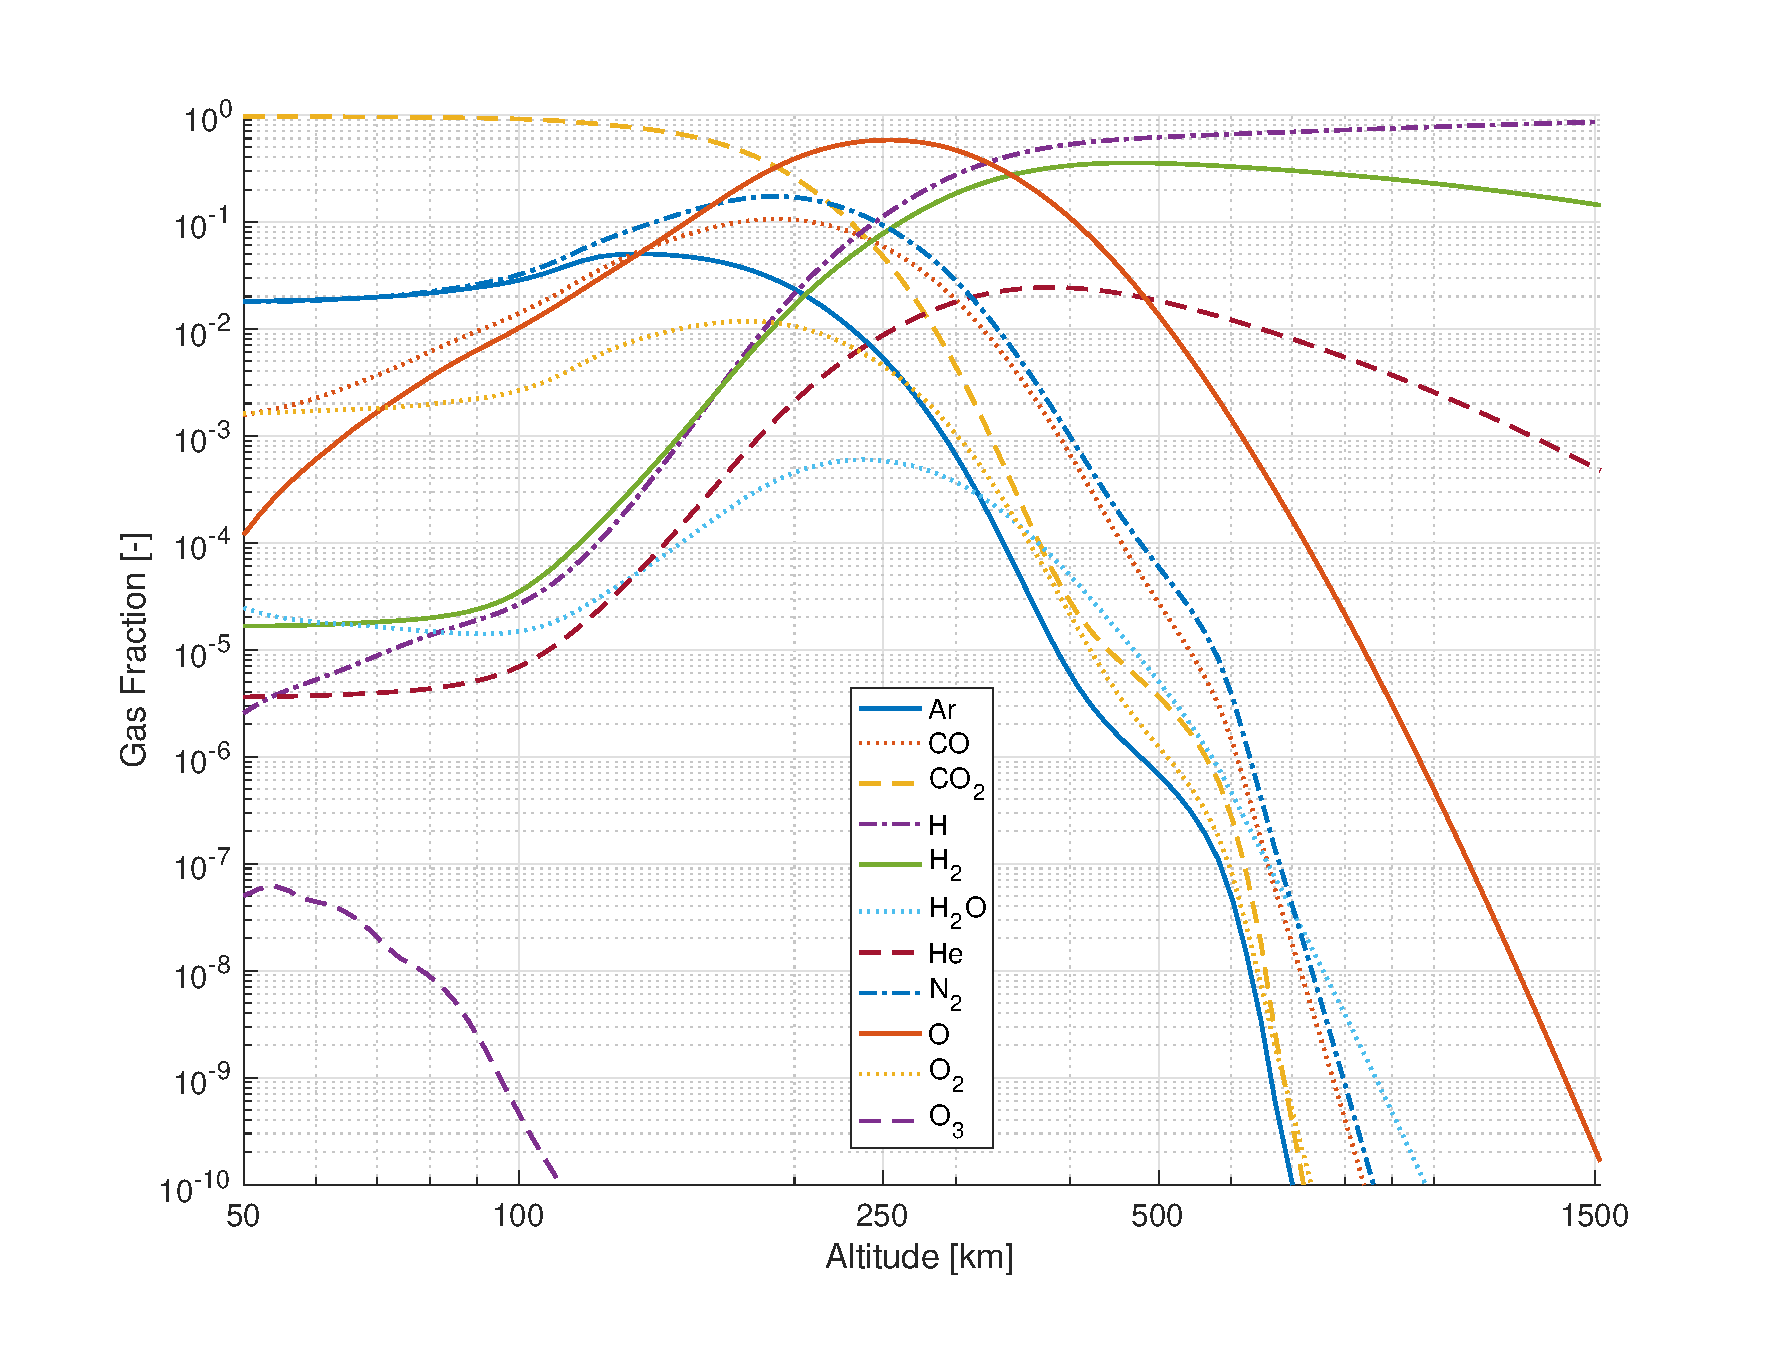
\includegraphics[width=0.7\textwidth]{figures/composition}
	\caption[This is an example figure. You can also refer to the author of this figure.]{This is an example figure. You can also refer to the author of this figure~\citep{MST001}. This figure, by the way, shows the gas concentrations as a function of altitude, for the atmosphere of Mars.}
	\label{fig:figure}
\end{figure}

\begin{table}[htb!]
	\centering
	\caption[This is an example table.]{This is an example table. Here one can see the effect of the custom table alignment options.}
	\label{tab:table}
	\begin{tabular}{ccC{2cm}}
		\toprule
		\textbf{Column 1} & \textbf{Column 2} & \textbf{Column 3} \\
		\midrule
		$x$ & 10 & Some very long text that is constrained in width by the \verb|C{}| alignment option to \SI{2}{\centi\meter} \\
		\bottomrule
	\end{tabular}
\end{table}

